\section{Online Analytical Processing (OLAP)} \label{section:olap}

El Procesamiento Anal\'itico en L\'inea (\textbf{OLAP}) es una tecnología de organización de grandes bases de datos 
comerciales que facilita a los usuarios el an\'alisis de grandes conjuntos de datos multidimensionales de manera 
eficiente y efectiva. A diferencia de las bases de datos relacionales tradicionales, que se centran en el procesamiento 
de transacciones y la actualización de datos en tiempo real, OLAP se enfoca en el análisis de datos históricos y la 
identificación de patrones y tendencias. 

\subsection{Objetivos de los sistemas OLAP}

En términos generales, el objetivo principal de OLAP es proporcionar una plataforma para el análisis de datos 
multidimensionales de manera eficiente y efectiva. De forma m\'as espec\'ifica OLAP tiene el objetivo de: 

\begin{itemize}
    \item Brindar a los analistas de datos flexibilidad a la hora de realizar sus labores, permitiendoles analizar los datos desde 
        diferentes perspectivas y dimensiones, así como la capacidad de agregar o desagregar los datos según sea necesario.
    \item Ofrecer an\'alisis de forma r\'apida y eficiente, incluso cuando se manejan grandes cantidades de datos.
    \item Ser fácilmente accesible para los usuarios finales, incluso si no tienen experiencia en programación o en el 
        manejo de bases de datos. Esto se logra a través de interfaces de usuario intuitivas y herramientas de análisis 
        visuales que permiten a los usuarios explorar los datos de manera interactiva.
    \item Ser f\'acilmente integrable con otras aplicaciones de análisis y reporting, lo que permite a las organizaciones 
        utilizar la tecnología en conjunto con otras herramientas de análisis de datos y visualización.
    \item Otorgar seguridad permitiendo a las organizaciones controlar quiénes tienen acceso a los datos y qué acciones 
        pueden realizar. Esto es especialmente importante en el caso de datos confidenciales o críticos para el negocio.
\end{itemize}

\subsection{Arquitectura de los sistemas OLAP}

La arquitectura de un sistema OLAP consiste en múltiples componentes que trabajan en conjunto para brindar un entorno 
analítico integral. Estos son los componentes fundamentales de un sistema OLAP:

\subsubsection{Fuentes de Datos:}
El primer componente de un sistema OLAP son las fuentes de datos. Estas pueden ser cualquier número de diferentes 
tipos de fuentes de datos, como bases de datos relacionales o archivos planos. Las fuentes de 
datos son típicamente el punto de partida para el proceso ETL (Extraci\'on, Transformaci\'on, Carga), que extrae datos 
de los sistemas fuente y los carga en el sistema OLAP.

\subsubsection{ETL:}
El siguiente componente son los procesos ETL. Estos son los procesos que hacen posible 
que los datos sean extra\'idos de los sistemas fuente, se transformen en el formato requerido por el sistema OLAP y luego se 
cargan en el sistema OLAP. Los procesos ETL son los responsables de garantizar la calidad y consistencia de los datos, 
así como de realizar cualquier limpieza o agregación de datos necesarios.

\subsubsection{Almacén de datos:}
El tercer componente de un sistema OLAP es el almacén de datos, Data Warehouse en ingl\'es. Aquí es donde se almacenan y 
organizan los datos de manera optimizada para consultas analíticas. M\'as adelante se profundizar\'a en las especificidades 
de los Almacenes de Datos.

\subsubsection{Motor OLAP:}
El motor OLAP es el responsable de responder consultas analíticas de forma rápida y eficiente sobre 
los datos en el almacén de datos. El motor OLAP consiste en un conjunto de algoritmos y estructuras de datos 
optimizadas para consultas analíticas, como cubos multidimensionales, índices de bits y esquemas en estrella.

\subsubsection{Herramientas de cliente:}
El último componente de un sistema OLAP son las herramientas de cliente. Estas son las herramientas que utilizan los 
usuarios finales para interactuar con el sistema OLAP y realizar consultas analíticas. Las herramientas de cliente pueden 
incluir desde simples paneles basados en web hasta herramientas sofisticadas de visualización y análisis de datos.

\subsection{Almacenes de datos}

El término \emph{Data Warehouse} fue acuñado por primera vez por Bill Inmon en 1990. William H. Inmon planteó que: 
“Un \textbf{\emph{Data Warehouse}} es una colección de datos integrada, orientada a sujetos, variante en el tiempo y 
no volátil, utilizada como apoyo para los procesos de toma de decisión.”

Analizando cada uno de los elementos principales de esta definición, se puede obtener una mejor comprensión de qué es un 
almacén de datos:

\subsubsection{Orientados a sujetos:}
%
Hace referencia a un sistema que est\'a organizado en base a temas o conceptos especiales, permitiendo que los datos y la 
información de un mismo tipo quede siempre conectada.

\subsubsection{Integrados:}
Los datos se obtienen de fuentes diferentes, por ejemplo de los diferentes departamentos de una organización, por lo que se 
deben aplicar técnicas que permitan determinar las interrelaciones existentes entre los datos, para luego guardarlos en el 
almacén y que puedan ser accedidos eficientemente durante las consultas.

\subsubsection{No Vol\'atiles:}
La información contenida en un almac\'en de datos existe para ser leída, pero no modificada.

\subsubsection{Variables con el tiempo:}
Los cambios producidos en los datos a lo largo del tiempo quedan registrados, para que los informes que se generen reflejen 
esas variaciones.


No se puede hablar de Almacenes de Datos sin mencionar los modelos dimensionales. A trav\'es de los a\~{n}os, la industria 
a conclu\'ido que el modelado dimensional es la t\'ecnica m\'as apropiada para entregar datos a los usuarios de los 
almacenes de datos. En la siguiente sección profundizaremos en el modelo dimensional.

\subsection{Modelo Dimensional}

Un modelo dimensional contiene la misma información que un modelo normalizado, pero empaqueta los datos en un formato 
distinto, que tiene como objetivos de diseño la comprensión del usuario, el rendimiento de las consultas y la resiliencia 
al cambio. Un modelo dimensional se compone de dos elementos fundamentales: las tablas de hechos y las tablas de dimensi\'on.
%
\subsubsection{Tablas de Hechos: }
%
Una tabla de hechos es la tabla principal en un modelo dimensional, en la cual se almacenan las mediciones de desempeño del 
negocio, generalmente valores num\'ericos\cite{kimball2011data}. Una fila en una tabla de hechos corresponde a una medida.
%
\begin{figure}[ht]
    \centering
    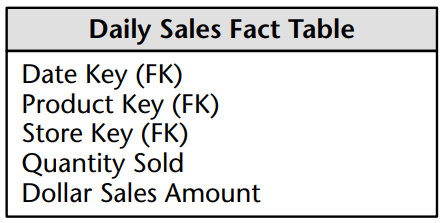
\includegraphics[width=0.5\textwidth]{../document/Graphics/hechos.png}
    \caption{Tabla de Hechos Daily Sales (Ventas Diarias) \cite{kimball2011data}}
    \label{fig:facts}
  \end{figure}
%

La Figura\ref{fig:facts} muestra un ejemplo de una tabla de hechos que contiene datos sobre las ventas de un producto, en una fecha dada, 
en una tienda determinada. N\'otese que los atributos Quantity Sold (Cantidad Vendida) y Dollar Sales Amount (Cantidad de 
Ventas en Dólares), son atributos num\'ericos que pueden ser de gran ayuda para analizar la rentabilidad y otros indicadores 
del negocio. 

Las tablas de hechos normalmente ocupan el $90\%$\cite{kimball2011data} del espacio de las bases de datos dimensionales, por tanto, 
los desarrolladores deben tener bien en cuenta el espacio que ocupa la tabla. Es inconveniente almacenar 
registros num\'ericos que no vayan a aportar nada relevante a los an\'alisis. Esto tambi\'en se aplica para los atributos 
de tipo texto, ya que ocupan mayor espacio que los datos num\'ericos y por su naturaleza heterog\'enea es conveniente 
mantenerlos fuera de las tablas de hechos; aunque esto no es absoluto\cite{kimball2011data}.

Las tablas de hechos contienen dos o m\'as llaves for\'aneas, que conectan con las llaves primarias de las tablas de 
dimensiones.
%
\subsubsection{Tablas de Dimensiones: }
%
Las tablas de dimensiones contienen los descriptores textuales del negocio. Cada dimensión se identifica por su llave 
primaria, la cual es \'unica y sirve como base para asegurar la integridad referencial en cualquier tabla de hechos con 
la que se interrelaciona. Los atributos de las tablas de dimensi\'on son la fuente fundamental de restricciones en las 
consultas al modelo dimensional, son fundamentales para hacer que el almacén de datos sea utilizable y comprensible. Las 
dimensiones implementan la interfaz de usuario para el almacén de datos, por tanto, cuánto más tiempo se dedique a 
proporcionar atributos con información detallada y terminología comercial, mejor es el almacén de datos.

\begin{figure}[ht]
    \centering
    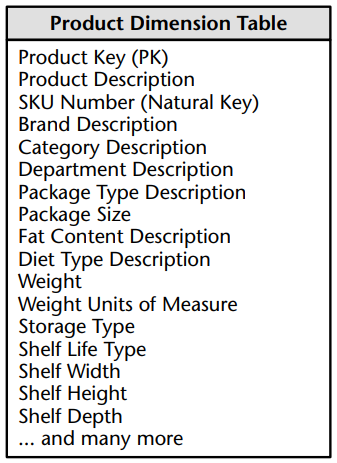
\includegraphics[width=0.5\textwidth]{../document/Graphics/dimension.png}
    \caption{Tabla de Dimensi\'on Producto \cite{kimball2011data}}
    \label{fig:dimension}
  \end{figure}

La Figura\ref{fig:dimension} muestra un ejemplo de la tabla de la dimensi\'on Product (Producto). 
%
\subsubsection{Esquema Estrella y Esquema Copo de Nieve: }

Las tablas de hechos y tablas de dimensiones se combinan para formar un modelo dimensional. Como se puede observar en la 
Figura\ref{fig:dimmodel}, la tabla de hechos Ventas, que almacena las medidas de inter\'es, se encuentra en el centro del esquema, 
interrelacionada a las tablas de dimensiones, que le proporcionan a las medidas atributos descriptivos.

\begin{figure}[ht]
  \centering
  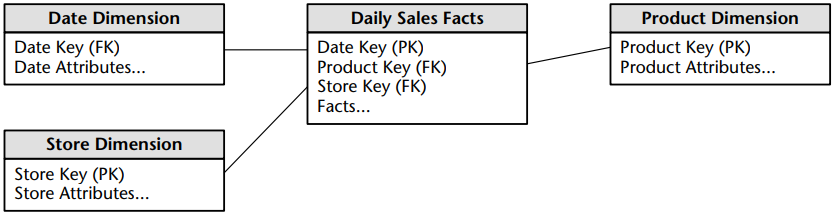
\includegraphics[width=1\textwidth]{../document/Graphics/star schema.png}
  \caption{Modelo Dimensional \cite{kimball2011data}}
  \label{fig:dimmodel}
\end{figure}

A esta estructura se le conoce como Esquema Estrella (\emph{Star Schema}). Debido a su simplicidad, son f\'aciles de leer 
y de comprender los procesos que intentan modelar. Adem\'as tienen un rendimiento sobresaliente, con pocas operaciones se 
pueden manejar consultas complicadas sobre los hechos. Sin embargo, tienen una deficiencia, con tal de mantener la 
simplicidad, permiten redundancia de datos en las tablas de dimensiones.

Ejemplo de esto es la tabla de la dimensi\'on Product, Figura\ref{fig:dimension}. N\'otese que se puede almacenar varios productos de una 
misma marca, por tanto, la información de Brand Descriptor (Descriptor de Marca) se repetir\'ia por cada producto de la 
misma marca. Lo mismo sucede con Category Description (Descriptor de Categor\'ia) y otros de los atributos. Es decir, la 
información en esta tabla ser\'a redundante. Sin embargo, con el objetivo de optimizar el rendimiento de las consultas y 
de mantener la legibilidad del modelo, se abstiene de crear una tabla aparte con la informaci\'on de las marcas, y unirla 
a la dimensi\'on Product mediante una llave for\'anea. Si se realiza esta transformaci\'on en las tablas de dimensi\'on, 
el Esquema Estrella converge al Esquema Copo de Nieve (\emph{Snowflake Schema}).

En el esquema Copo de Nieve, las dimensiones se encuentran normalizadas en varias tablas relacionales. El efecto Copo de Nieve solo afecta a las tablas de 
dimensiones, las tablas de hechos permanecen iguales que en el Esquema Estrella, en el centro del modelo. La ventaja de este esquema es que puede ayudar a reducir 
la redundancia y mejorar la integridad de los datos. Sin embargo, en este esquema las consultas pueden resultar menos eficientes que en el Esquema Estrella, debido 
a que intervienen un mayor número de tablas en las operaciones. Adem\'as, el Esquema Copo de Nieve puede resultar m\'as dif\'icil de entender y mantener, pues incrementa la complejidad del 
dise\~{n}o del modelo.

La decisi\'on de usar uno u otro esquema depende de los requerimientos espec\'ificos del proyecto y de las compensaciones entre rendimiento de las consultas, 
la complejidad del esquema y la integridad de los datos.


\subsection{Arquitectura de un almac\'en de datos}

La estructura de un Almac\'en de Datos puede ser separada por capas. Aunque esto es un tema pol\'emico. Los mismos Inmon y Kimball tienen posiciones dispares 
con respecto a este tema. Seg\'un Inmon los Data Marts est\'an f\'isicamente separados del Almac\'en de Datos y la forma de acceder a los datos es a trav\'es de los Data Marts \cite{inmon}.
Por otro lado, Kimball no concibe esta separaci\'on y los usuarios acceden a los datos del almac\'en directamente \cite{kimball2011data}.

Cada autor propone diferentes nombres para las capas, pero de manera general pueden distinguirse 3 capas:

\subsubsection{Sistemas Operacionales:}
Son las fuentes de datos primarias del Almac\'en de Datos.

\subsubsection{Almac\'en de Datos Empresarial:} 
Es la capa fundamental del almac\'en. Almacena los datos reconciliados, extra\'idos de los sistemas operacionales. De acuerdo con Kimball esta capa est\'a compuesta
por los datos integrados de los distintos Data Marts. En cambio, seg\'un Inmon es una estructura en tercera forma normal y los Data Marts derivados, separados f\'isicamente. 

\subsubsection{Capa de Reportes:} Es donde los usuarios interact\'uan con el Almac\'en de Datos.

\subsection{Herramientas OLAP}

En el campo del Procesamiento Analítico en Línea (OLAP), existen varias herramientas y plataformas establecidas que 
proporcionan capacidades sólidas para el análisis de datos y el apoyo a la toma de decisiones. Estas herramientas ofrecen 
una amplia gama de características y funcionalidades para empoderar a las organizaciones en la obtención de conocimientos a 
partir de sus datos. A continuaci\'on discutiremos algunas de las m\'as conocidas: 

\subsubsection{Microsoft SQL Server Analysis Services (SSAS): }

Microsoft SQL Server Analysis Services (SSAS) es una herramienta OLAP que forma parte del conjunto de herramientas 
de Microsoft SQL Server. Brinda capacidades de análisis multidimensionales y minería de datos, permitiendo a los 
usuarios crear y gestionar cubos OLAP para un análisis avanzado de datos. SSAS admite tanto el modelo multidimensional 
como el modelo tabular, brindando flexibilidad en la modelización y consultas de datos.

\subsubsection{Oracle Essbase: }

Oracle Essbase es una herramienta OLAP ofrecida por Oracle Corporation. Proporciona un sistema de gestión de bases de datos 
multidimensionales que permite realizar análisis y pronósticos complejos. Admite diversas técnicas de modelado de datos, incluyendo 
dimensiones densas y dispersas, así como capacidades avanzadas de cálculo. Essbase se integra con otras herramientas y 
plataformas de Oracle, ofreciendo una solución integral para análisis empresarial.

\subsubsection{IBM Cognos TM1: }

IBM Cognos TM1 es una potente herramienta OLAP diseñada para la gestión del rendimiento y la planificación. Permite a las 
organizaciones crear modelos multidimensionales y realizar análisis en tiempo real de datos financieros y operativos. TM1 
ofrece un entorno dinámico y flexible para presupuestar, pronosticar y modelar escenarios. Proporciona capacidades 
avanzadas de consolidación de datos, análisis "what-if" y análisis predictivo. TM1 se integra con otras herramientas de 
IBM Cognos, mejorando las capacidades generales de inteligencia empresarial.

\subsubsection{Pentaho Mondrian: }

Pentaho Mondrian es un servidor OLAP de código abierto que forma parte de la plataforma de análisis empresarial Pentaho. 
Permite a los usuarios la creación e implementaci\'on de cubos OLAP para el análisis interactivo de datos. Mondrian es 
compatible con el lenguaje de consulta MDX (Multi-Dimensional eXpressions) y proporciona una interfaz basada en web 
para consultar y explorar datos. Ofrece características que permiten la navegaci\'on en datos multidimensionales como 
desglose, segmentación y pivotar. Mondrian se integra con otras herramientas de Pentaho, brindando una 
suite integral para la integración de datos, informes y análisis.
